\documentclass[a4paper, 12pt]{article}%тип документа

%%%Библиотеки
	%\usepackage[warn]{mathtext}	
	\usepackage[T2A]{fontenc} % кодировка
	\usepackage[utf8]{inputenc} % кодировка исходного текста
	\usepackage[english,russian]{babel} % локализация и переносы
	\usepackage{caption}
	\usepackage{listings}
	\usepackage{amsmath,amsfonts,amssymb,amsthm,mathtools}
	\usepackage{wasysym}
	\usepackage{graphicx}%Вставка картинок правильная
	\usepackage{float}%"Плавающие" картинки
	\usepackage{wrapfig}%Обтекание фигур (таблиц, картинок и прочего)
	\usepackage{fancyhdr} %загрузим пакет
	\usepackage{lscape}
	\usepackage{xcolor}
	\usepackage[normalem]{ulem}
	\usepackage{hyperref}

%%%Конец библиотек




%%%Настройка ссылок
	\hypersetup
	{
		colorlinks=true,
		linkcolor=blue,
		filecolor=magenta,
		urlcolor=blue
	}
%%%Конец настройки ссылок


%%%Настройка колонтитулы
	\pagestyle{fancy}
	\fancyhead{}
	\fancyhead[L]{Лабораторная работа}
	\fancyhead[R]{Талашкевич Даниил, группа Б01-009}
	\fancyfoot[C]{\thepage}
%%%конец настройки колонтитулы



							\begin{document}
						%%%%Начало документа%%%%


%%%Начало титульника
\begin{titlepage}

	\newpage
	\begin{center}
		\normalsize Московский физико-технический институт \\(госудраственный 			университет)
	\end{center}

	\vspace{6em}

	\begin{center}
		\Large Лабораторная работа по оптике\\
	\end{center}

	\vspace{1em}

	\begin{center}
		\large \textbf{Изучение призмы с помощью гониометра [4.4.3]}
	\end{center}

	\vspace{2em}

	\begin{center}
		\large Талашкевич Даниил Александрович\\
		Группа Б01-009
	\end{center}

	\vspace{\fill}

	\begin{center}
	Долгопрудный \\2022
	\end{center}
	
\end{titlepage}
%%%Конец Титульника



%%%Настройка оглавления и нумерации страниц
	\thispagestyle{empty}
	\newpage
	\tableofcontents
	\newpage
	\setcounter{page}{1}
%%%Настройка оглавления и нумерации страниц


					%%%%%%Начало работы с текстом%%%%%%

\section{Аннотация}

$\text{ }$

\textbf{Цель работы:} знакомство с работой гониометра, исследование дисперсии стеклянной призмы и определение характеристик призмы как спектрального прибора.
	
\textbf{В работе используются:} гониометр, ртутная лампа, призма, стеклянная плоскопараллельная пластинка, призменный уголковый отражатель.

\section{Теоретическое введение} 
	Гониометр служит для точного измерения углов и находит широкое применение в оптических лабораториях. С помощью гониометра можно определять показатели преломления и преломляющие углы призм и кристаллов, исследовать параметры дифракционных решёток, измерять длины волн спектральных линий и т. д. В настоящей работе прибор применяется для исследования дисперсии стеклянных призм --- зависимости показателя преломления от длины волны.
	\begin{figure}[!h]
		\begin{center}
			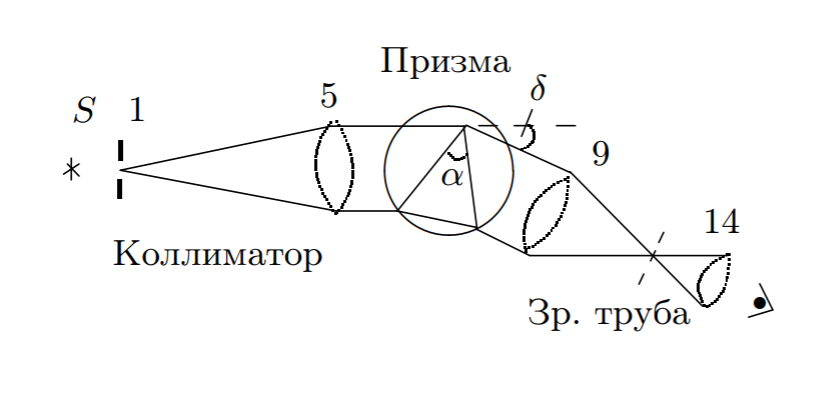
\includegraphics[width = 0.55\textwidth]{pic/443-1.png}
			\caption{Оптическая схема эксперимента}
		\end{center}
	\end{figure}
	Показатель преломления материала призмы удобно определять по углу наименьшего отклонения. Известно, что минимальное отклонение луча, преломленного призмой, от направления луча, падающего на призму, получается при симметричном ходе луча (в призме луч идёт перпендикулярно биссектрисе преломляющего угла). Угол минимального отклонения $\delta$, преломляющий угол $\alpha$ (угол при вершине призмы на рис. 1) и показатель преломления $n$ связаны между собой соотношением
	\begin{equation}
	n=\dfrac{\sin\dfrac{\alpha+\delta}{2}}{\sin\dfrac{\alpha}{2}}.
	\end{equation}
	Измерив с помощью гониометра преломляющий угол призмы и углы наименьшего отклонения для света разных длин волн, можно рассчитать величину $n$ и построить дисперсионную кривую --- график зависимости $n(\lambda)$. 
	
	По дисперсионной кривой могут быть определены такие важные характеристики оптических стёкол, как средняя дисперсия
	\begin{equation}
	D = n_F - n_C
	\end{equation}
	и коэффициент дисперсии $\nu$ (число Аббе):
	\begin{equation}
	\nu = \dfrac{n_D - 1}{n_F - n_C},
	\end{equation}
	где $n_D, n_F$ и $n_C$ --- показатели преломления для $\lambda_D = 589{,}3$ нм (среднее значение длин волн жёлтого дублета натрия), $\lambda_F = 486{,}1$ нм (голубая линия водорода), $\lambda_C = 656{,}3$ нм (красная линия водорода).
	
	По наклону дисперсионной кривой можно оценить разрешающую
	способность призмы
	\begin{equation}
	R = \dfrac{\lambda}{\delta\lambda} = b\dfrac{dn}{d\lambda}.
	\end{equation}
	Здесь $\delta\lambda$ --- минимальный интервал длин волн, разрешаемый по критерию Релея, $b$ --- размер основания призмы, если вся рабочая грань призмы освещена параллельным пучком.
	
		\begin{figure}[!h]
		\begin{center}
			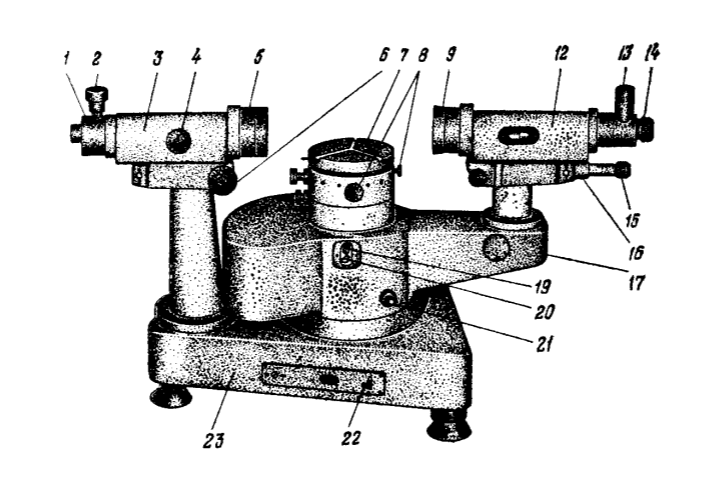
\includegraphics[scale = 0.5]{pic/443-2.png}
			\caption{Внешний вид гониометра}
		\end{center}
	\end{figure}

\section{Экспериментальная установка}

\section{Ход работы}

\section{Вывод}

\section{Литература}

\begin{enumerate}

\item Лабораторный практикум по общей физике. В 3 т. Том 2. Оптика: учебное пособие

\item http://mathhelpplanet.com (МНК и регрессионный анализ)


\end{enumerate}	

\end{document}
